\documentclass[final]{summery_5.0}
\title{Experimentalphysik Vb - Teilchenphysik\\Zusammenfassung}
\date{WS 24/25}

\begin{document}
\maketitle
\tableofcontents

\part{Teilchenphysik}
\section{Wiederholung}

\subsection{Streumessungen}
Bei einem Streuexperiment werden Teilchen der Energie \(E_0=mv_0^2/2\) mit der Teilchendichte \(n\) [m${}^{-3}$] und der Teilchenflussdichte \(\Phi=n\cdot v_0\) auf ein Target mit Teilchendichte \(n_T\) und Target Volumen \(V = F\cdot \Delta x\), mit der Querschnittsfläche \(F\) und der Dicke \(\Delta x\), geschossen. Auf die Querschnittsfläche treffen dann \(N=\Phi\cdot F\) Teilchen pro Sekunde. Für elastische Streuung gilt:

\begin{empheq}{align*}
    \frac{\Delta N}{N} &= f(\theta,E_0) \Delta \Omega\\
    f(\theta,E_0) &= \frac{n_T V}{F} \dd \sigma \Omega (\theta,E_0) 
\end{empheq}
Der differenzielle Wirkungsquerschnitt \(\dd \sigma \Omega\) gibt den Beitrag eines Targetkerns zur Streuung um den Winkel \(\theta\) in den Raumwinkel \(\Omega\) an.

\subsection{Relativistische Formeln}
Das Quadrat des Energie-Impuls-Vektors liefert den Zusammenhang
\begin{align*}
    \boxed{E = \sqrt{c^2p^2 + m_0^2 c^4}}
\end{align*}
Teilchen die nicht die Energie-Impuls-Relation erfüllen, nennt man \glqq offshell\grqq, es sind sogenannte virtuelle Teilchen. 

Es sei das Verhältnis von kinetischer Energie zu Ruheenergie definiert als \(\alpha\). Viele Zusammenhänge lassen sich mithilfe von \(\alpha\) unabhängig von der Teilchenart schreiben:
\begin{empheq}{align*}
    p^\mu &= \hug{E/c, \v p }\\
    p_\mu p^\mu &= E^2- p^2\\
    \alpha &= \frac{E\sub{kin}}{m_0c^2} = \gamma - 1\\
    E\sub{kin} &= E-m_0 c^2\\
    \v v &= \frac{c}{1+\alpha}\sqrt{\alpha^2 + 2\alpha}\\
    \v p &= \gamma m v = \beta E\\ 
    \absv p &= m_0 c \sqrt{\alpha^2 + 2\alpha}\\ 
    \lambda &= \frac hp= \frac h {m_0 c \sqrt{\alpha^2 + 2\alpha}}\\
    \gamma &= \frac{E}{m_c c^2}\\
    \beta  &= \frac{p c}{E}
\end{empheq}

\section{Natürliche Einheiten}
Für eine übersichtlichere Notation bedient man sich den natürlichen Einheiten, welche man durch folgenden Definitionen erhält:
\begin{align*}
    \boxed{\hbar\equiv c\equiv \epsilon_0 \equiv k_B \equiv 1}
\end{align*}
Es folgt eine Tabelle der neuen Größen und Umrechnungsfaktoren.
\begin{table}[H]
    \centering
    \sisetup{table-format = 1.2e+2{$\u{N\,s}$}}
    \begin{tabular}{@{}lccS@{}}
        \toprule
        {\bf Größe}& \multicolumn{2}{c}{{\bf Einheit}} & {\bf Wert in SI} \\
        \cmidrule(lr){2-3} 
        & geschrieben & tatsächlich & \\
        \midrule
        Energie & \(1\u{eV}\) &  & 1.60e-19{\,\si\J}\\
        Masse & \(1\u{eV}\) & \(\frac{1\u{eV}}{c^2}\) & 1.78e-36{\,\si\kg}\\
        Impuls & \(1\u{eV}\) & \(\frac{1\u{eV}}{c}\) & 5.34e-28{$\u{N\,s}$}\\
        Temperatur & \(1\u{eV}\) & \(\frac{1\u{eV}}{k_B}\) & 1.16e4 {$\u K$}\\  
        Zeit & \(1/\u{eV}\) & \(\frac\hbar{1\u{eV}}\) & 6.58e-16 {$\u s$}\\
        Länge & \(1/\u{eV}\) & \(\frac{c\hbar}{1\u{eV}}\) & 1.97e-7 {$\u m $}\\
        \bottomrule
    \end{tabular}
\end{table}

Ein sehr nützlicher Zusammenhang zum Umrechnen zwischen Einheiten ist, dass
\begin{align*}
    \Aboxed{\hbar c \approx 197\u{MeV}\cdot \te{fm}}
\end{align*}

\section{Streureaktionen}
Streureaktionen sind Reaktionen von Teilchen der Form \(P_1+P_2\to P_3+P_4\). Zur Beschreibung werden die sogennanten Mandelstam-Variablen verwendet (Definition mit Minkowski-Tensor $\diag(1,-1,-1,-1)$): 
\begin{itemize}
    \item Quadrat der Schwertpunktsenergie: $s\equiv (p_1+p_2)^2 = (p_3+p_4)^2$
    \item Quadrat der Viererimpuls-Übertragung: $t\equiv (p_1-p_3)^2=(p_2-p_4)^2$
    \item Viererimpuls-Übertrag auf das Rückstoßteilchen: $u\equiv (p_1-p_4)^2 = (p_2-p_3)^2$
\end{itemize}
Die drei Variablen sind nicht unabhängig, es gilt zwischen ihnen die nützliche Beziehung:
\begin{align*}
    s+t+u &= \sum_i m_i^2
\end{align*}

\subsection{Streukanäle}
Es gibt drei typische Streukanäle, $s$ (timelike), $t$ und $u$ (beide spacelike). Sie werden durch die jeweilige Mandelstam-Variable charakterisiert, welche den quadrierten Viererimpuls des (virtuellen) Austauschteilchens beschreibt. 
\begin{description}
    \item[$s$-Kanal:] Nur beim s-Kanal können neue reelle Teilchen entstehen. $s$ beschreibt das Quadrat der Schwertpunktsenergie.
    
    \begin{figure}[H]
        \centering
        \includesvg[width=.2\textwidth]{s-channel.svg}
    \end{figure}

    \item[$t$-Kanal:] \,
    $t$ beschreibt das Quadrat des Viererimpuls-Übertragts.
    \begin{figure}[H]
        \centering
        \includesvg[width=.2\textwidth]{t-channel.svg}
    \end{figure}
    
    \item[$u$-Kanal:] \,
    $u$ beschreibt das Quadrat des Viererimpuls-Übertrags auf das Rückstoßteilchen.
    \begin{figure}[H]
        \centering
        \includesvg[width=.2\textwidth]{u-channel.svg}
    \end{figure}
    Der $u$-Kanal ist praktisch identisch zum $t-$Kanal, nur dass die End-Teilchen Plätze tauschen. Bei identischen Teilchen müssen daher immer $t$- und $u$-Kanal berücksichtigt werden.
\end{description}

\subsection{Elektromagnetische Streureaktionen}
\begin{itemize}
    \item{\bf Elektron Muon Streuung}: $e^- \mu^- \to e^- \mu^-$
    \item {\bf Bhabha-Streuung:} $e^+ e^- \to e^+ e^-$, $s$ und $t$ Kanäle
    \item{\bf Møller-Streuung:} $e^- e^- \to e^- e^-$
    \item $e^+ e^- \to \mu^+ \mu^-${\bf-Streuung:} Es gibt hier keinen t-Kanal, da Leptonen an einzelnen Vertizes aufgrund der
    Leptonzahlerhaltung nicht in Leptonen anderer Generationen umgewandelt
    werden können
    \item{\bf Compton-Effekt:} Die Wellenlänge des gestreuten Photons ergibt sich mit dem Streuwinkel \(\theta\) durch:
    \begin{align*}
        \lambda ' = \lambda + \frac h{m_e c} (1-\cos\theta)
    \end{align*}
\end{itemize}

\section{Teilchenbeschleuniger}
Zur Auflösung von Strukturen von z.B. eines Atomkerns muss die De-Broglie Wellenlänge \(\lambda= h / p\) klein sein gegenüber des Targetdurchmessers.
Um ausreichend große Energien zu erreichen, beschleunigt man geladene Teilchen in elektromagnetischen Feldern. Eine Tabelle aller wichtigen Teilchenbeschleunigern findet sich unter \url{https://en.wikipedia.org/wiki/List_of_accelerators_in_particle_physics#Colliders}. Der wichtigste und leistungsstärkste ist der Large Hadron Collider (LHC) in Cern. In dem 27km langen Teilchenbeschleuniger an vier verschienden Stellen haubtsächlich Proton-Proton-Kollisionen erzeugt und vermessen.

\subsection{Typen}
\begin{itemize}
    \item {\bf Linearbeschleuniger:}
    Ein Linearbeschleuniger beschleunigt Teilchen, indem sie in ein E-Feld geleitet werden, und zur Blende hin beschleunigt werden. Natürlich können mehere Linearbeschleuniger hintereinandergeschaltet werden, sodass die Höhstenenergie nur durch die praktikable Länge des Beschleunigers beschränkt ist. 
    Bei einem Driftröhren Beschleuniger wird eine hochfrequente Spannung $U(t) = U_0 \sin(\omega t)$ angelegt, und die Längen $l_i$ der Röhren wird so gewählt, dass die Teilchen immer nach einer halben Periode der Wechselspannung in den nächsten Zwischenraum gelangen $l_i= \frac{v_i}{2f} $. Der Energiezuwachs in jedem Zwischenraum ist \(\Delta E= q U_0 \sin\Psi_s\), wobei $\Psi_s$ die mittlere Sollphase ist, zu der die Teilchen jeweils die Zwischenraumume passieren.
    \begin{figure}[H]
        \centering
        \includegraphics[width=0.5\textwidth]{linear_beschleuniger.png}
    \end{figure}
    Tatsächlich verwendet man nicht den Maximalwert der Beschleunigungspannung, sondern die ansteigende Flanke. Dies fokossiert die Phase, denn zu schnelle Teilchen erfahren ein kleineres Feld, und zu langsame ein stärkeres.

    \item{\bf Alvarez-Strukturen:}
    Alvarez-Strukturen sind im wesentlichen moderne Linearbeschleuniger, die stehende elektromagentische Wellen zur Beschleunigung verwenden. 

    \item{\bf Kreisbeschleuniger:}
    Der Kreisbeschleuniger ist praktisch ein aufgerollter Linearbeschleuniger, wobei die Ladungsträger mit B-Feldern auf der Kreisbahn gehalten werden. Man unterscheidet zwischen Zyklotrons $\omega_Z = \frac{qB_\perp}{m}$, bei denen das B-Feld konstant ist, und sich die Teilchen auf Kreisbahnen mit variablen Radien bewegen, und Synchrotrons, bei denen die Kreisbahn der Teilchen konstant ist, und dafür das B-Feld variiert wird. Klassische Zyklotrons beschleunigen auf rund $\SI{20}{MeV}$ pro Ladungseinheit, Synchrotrons kommen bis weit über $1000\u{GeV}$. Da der Energieverlust durch Synchrotronstrahlung $\Delta E \sim \frac{E^4}{rm^4}$ für Protonen um einen Faktor $\sim10^{-14}$ kleiner ist im Vergleich zu Elektronen kommen am LHC nur schwere Teilchen zum Einsatz. 

    Aus Gleichsetzen von Zentripetalkraft und Lorentzkraft folgt für den Radius:
    \begin{align*}
        r = \frac p {qB_\perp}
    \end{align*}
\end{itemize}

\subsection{Strahlführung}
Der Teilchenstrahl wird in Kreisbeschleunigern auf der Bahn gehalten, indem Quadrupolmagneten angelegt werden. Mit einem Quadrupolmagneten ist das B-Feld
\begin{align*}
    \v B = g \colvec{y}x0
\end{align*}
und führt somit bei einer Abweichung in $x$-Richtung zur Lorentzkraft
\begin{align*}
    \v F &= e\, \v v \times \v B = ecg\colvec{-x}{y}{0}\\
\end{align*}
welche den Strahl in $x$-Richtung fokossiert, und in $y$-Richtung zerstreut. Durch Kombination von zwei um $90^\circ$ gedrehte Magneten erhält man die gewünschte Fokossierung in $x-$ und $y$-Richtung. 



\subsection{Luminosität}
Die Luminosität $L$ ist die zentrale Größe, welche beim Bau von Teilchenbeschleunigern optimiert wird, um eine möglichst große Ereignisrate $\dot N = L \sigma$ zu erreichen.

Allgemein ergibt sie sich durch ein Überlappungsintegral, mit $\rho_{1,2}$ als Dichtefunktionen der Teilchenstrahlen, und $s_0=ct$ als zeitlichen Abstand vom Wechselwirkungspunkt:
\begin{align*}
    \boxed{L = K N_1 N_2 f n_B \iiiint  \rho_1(x,y,s,-s_0)\rho_2(x,y,s,s_0) \dx \dy \d s \d s_0}
\end{align*}

Für einen Speicherring, in den $n_B$ bunches mit jeweiligen Teilchenzahlen $N_1$ und $N_2$ (zwei entgegenlaufende Strahlen) in der Frequenz $f$ umlaufen, gilt unter der Annahme eines gaußschen Strahlquerschnittes am Kollisionspunkt die folgende Gleichung:

\begin{align*}
    \boxed{L = \frac{n_B f N_1 N_2}{4\pi \sigma_x \sigma_y}}
\end{align*}

\subsection{Synchrotronstrahlung}
Ladungsträger, welche beschleunigt werden, strahlen jeden Umlauf eine Energiemenge $\Delta E$ ab:
\begin{align*}
    \boxed{\te{\bf Lamor-Formel:}\quad \Delta E = \frac{4\pi \alpha\hbar c}{3} \frac{\gamma^4}{r}\propto \frac1 r \frac{E^4}{m^4}}
\end{align*}
Sehr hohe Energien sind somit leichter für schwere Teilchen erreichbar. Für den halben Öffungswinkel gilt $\theta \sim \frac1 \gamma$.

\section{Teilchendetektoren}

\subsection{Gemessene Teilcheneigenschaften}
\begin{itemize}
    \item {\bf Ort:} ergibt sich aus der Stelle im Detektor, an dem das Signal gemessen wurde.
    \item {\bf Energie:} wird gemessen über das Signal aus der vollständigen Absorbtion des Teilchens. 
    \item {\bf Impuls:} aus der Krümmung der Teilchenbahn im Magnetfeld.
    \item {\bf Geschwindigkeit:} entweder Flugzeitmessung, oder geschwindigkeitsabhängige Effekte: Energieverlust pro Strecke (BBF), Cherenkov-Strahlung, Übergangsstrahlung.
    \item {\bf Masse:} aus den Impuls und Geschwindigkeitsmessung.
    \item {\bf Ladungs:} aus dem Energieverlust pro Strecke (BBF), und das Vorzeichen durch die Krümmung der Flugbahn im B-Feld.
    \item {\bf Lebensdauer:} aus Messung der Zeit oder Flugstrecke zwischen Erzeugung und Zerfall.
    \item {\bf Vertex:} (Punkt der Erzeugung) durch Rückverfolgung der Teilchenbahn.
    \item {\bf Identität:} über die Messung der Masse und der Ladung.
\end{itemize}

\subsection{Elektromagnetische Wechselwirkungen}
    Zwischen Teilchen und Materie gibt es vier elektromagnetische Wechselwirkungen:
\begin{itemize}
    \item {\bf Ionisierung:} Die Teilchen Wechselwirken mit den Hüllenelektronen. Das Atom wird entweder angeregt oder Ionisiert.
    \item {\bf Bremsstrahlung:} WW mit den Atomkernen. Das einfallende Teilchen wird abgelenkt und emittiert Bremsstrahlung.
    \item {\bf Chrenkov-Strahlung:} Wenn das Teilchen schneller ist als die Lichtgeschwindigkeit in dem Medium strahlt es Cherenkov-Strahlung ab.
    \item {\bf Übergangsstrahlung:} Wenn das Teilchen Grenzflächen zwischen verschiedenen Materialien passiert, strahlt es Übergangsstrahlung ab. 
\end{itemize}

\subsection{Energieverluste}
\subsubsection{Elektronen/Positronen}
Leichte Teilchen wie Elektronen verlieren bei niedrigen Energien primär Energie über \emph{Ionisierung}. 

Ab einer kritschen Energie von 
\begin{align*}
    \Aboxed{E_c = \frac{560\u{MeV}}{Z}}
\end{align*}
verliert die Ionisierung an Bedeutung, da nun primär über \emph{Bremsstrahlung} Energie abgestrahlt wird. Mit der charakteristischen Strahlungslänge (Skintiefe) $x_0$ ist diese beschrieben durch:
\begin{align*}
    \Aboxed{-\hug{\dd Ex}\sub{Brems} &= \frac{1}{x_0}E \sim \underbrace{\frac{Z^2}A\ln\hug{\frac{183}{Z^\frac13}}}\sub{Absorbermaterial} \cdot \underbrace{\frac{z^2 E}{m^2}}\sub{Strahlteilchen}}
\end{align*}

\subsubsection{Schwere geladene Teilchen}
In einem Bereich von 
\begin{align*}
    \beta \gamma &= \frac pm \in[0.1, 1000]
\end{align*}
beschreibt die \emph{Bethe-Bloch-Formel} für \emph{schwere Teilchen} den mittleren Energieverlust durch \emph{Ionisierung und Stöße}.
\begin{align*}
    \boxed{\te{\bf Bethe-Bloch-Formel:}\quad \tug{-\dd Ex} 
    = \frac{K z^2 Z \rho }{A\beta^2} \bug{\ln \hug{\frac{2m_e e^2 \gamma^2 \beta^2}{I}} - \beta^2 - \frac\delta 2} \sim z^2}
\end{align*}
Hierbei sind: $K=4\pi N_A re^1 m_e c^2 = 0.307\u{MeV/g/cm}$aus verschiedenen Naturkonstanten zusammengesetzte Konstante, $\rho=$Dichte des Absorbers, $I=$ Ionisierungsenergie des Materials, $z=$ Ladungszahl der Strahlteilchen, $Z=$ Ladungszahl der Targetteilche, $\delta =$ Dichteffekt (materialabhängig).

Die BBF beschreibt den erwarteten Energieverlust, der wahrscheinlichste ist jedoch geringer ($\Delta E$ ist Landau verteilt).

Außerdem hat die BBF hat ein Minimum für $\beta\gamma\approx3.5$, dort gilt annähernd:
\begin{align*}
    \boxed{\te{\bf MIP:} \quad\frac1\rho \dd Ex \sim 2 \ufrac{MeV}{g/cm^2}}
\end{align*}

Der Energieverlust pro Strecke steigt stark an $\dd Ex \propto \frac1{\beta^2}$, es entsteht der Bragg-Peak.

Für sehr hohe Energien ($\sim50\u {GeV}$) dominiert wieder die Bremsstrahlung, siehe Energieverluste für Elektronen/Positronen.

\subsubsection{Hadronen}
Neben der Ionisation spielt für Hadronen die starke WW eine Rolle. Es entstehen Sekundärhadronen, welche wiederrum mit dem Medium wechselwirken. Es entsteht ein hadronischer Schauer. 

\subsubsection{Photonen}
Photonen wechselwirken abhängig von der Energie über den Photoeffekt ($E<1\u{MeV}$), den Comptoneffekt ($E\sim 1\u{MeV}$) und bei sehr hohen Energie über die Paarbildung ($E>1\u{MeV}$).
Für den Energieverlust ergibt sich ein Exponentialgesetz:
\begin{align*}
    \Aboxed{I = I_0 e^{-\mu x}\with \mu = \mu\sub{photo}+\mu\sub{compton}+\mu\sub{paar}}
\end{align*}

\subsubsection{Vielfachstreuung} 
Bei (wiederholter) Streuung ändert sich der Austrittswinkel des Teilchens relativ zum Eintrittswinkel. Für kleine Winkel ergibt sich ungefähr eine Gaußverteilung, die Ausläufer sind jedoch nicht gaußisch (Rutherford-Streuung). Für die Standardabweichung gilt:
\begin{align}
    \sigma_\theta &= \frac{13.6\u{MeV}}{\beta c p} z \sqrt{\frac x{X_0}} \bug{1 + 0.038 \ln\hug{\frac{x z^2}{X_0\beta^2}}}
\end{align}
mit $X_0$ als Strahlungslänge und $x$ als Dicke der Materialschicht.

\subsubsection{Cherenkov-Strahlung}
Passier ein geladenes Teilchen ein Medium mit Brechungsindex $n$ mit einer Geschwindigkeit $v>c/n$, so werden im Matrial Dipole induziert. Da die Geschwindigkeit größer als die Lichtgeschwindigkeit im Medium ist, ist die Rückstellung dieser Dipole gegenüber der Anregung neuer verzögert und es kommt zur Emission von Dipolstrahlung unter dem Winkel:
\begin{align*}
    \boxed{\cos(\theta_C) = \frac1{n\beta}}
\end{align*}
Dabei ist $\theta_C$ der Winkel zwischen der Ausbreitungsrichtung des Teilchens und der Wellenfront des ausgeandten Lichts.
Man bezeichnet Detektoreinheiten welche auf diesem Effekt beruhen  als RICH (ring imaging cherenkov detector).

\subsubsection{Übergangsstrahlung}
Bei dem Übergang zwischen zwei Medien mit unterschiedlicher Dielektrizitätskonstante muss ein
relativistisches Teilchen an der Grenzfläche elektromagnetische Strahlung abstrahlen. Es gelten dabei die Proportionalitäten:
\begin{align*}
    \Aboxed{\dd Et \sim \gamma,\qquad \theta \sim \frac1\gamma}
\end{align*}
Der Energieverlust durch Übergangsstrahlung
ist im Vergleich zu anderen Prozessen zu
vernachlässigen. Man bezeichnet Detektoreinheiten welche auf diesem Effekt beruhen  als TRD (transition radionation detector).

\subsubsection{}

\subsection{Konkrete Detektoren}
\subsubsection{Szintillatoren}
Bei einem Szintillator handelt es sich um ein Material, welches bei der Aufnahme von Energie dazu angeregt wird, Photonen zu emittieren. Die Anzahl der ausgelösten Photonen ist proportional zur Energie des einfallenden Teilchens,
Damit sich die Strahlung des Szintillators in diesem auch frei ausbreiten kann, ist des Material meist dotiert.

\subsubsection{Photomultiplier}
Ein Photomultiplier kann Photon-Signale in elektronische
Signale umwandeln. Dabei werden einerseits Kaskaden-Röhren, in denen durch
Photoeffekt Primärelektronen ausgelöst werden, welche dann durch Beschleunigung weitere Elektronen auslösen, oder Halbleiter-Photomultiplier eingesetzt. 

\subsubsection{Gasdetektoren}
In einem Gasdetektor wird ein Gas durch einfallende Strahlung ionisiert und die freien Ladungsträger dann durch ein elektrisches Feld beschleunigt und vermessen. Anhand der Flugdauer der Ionen und Elektronen kann man so die Spur des Teilchens nachvollziehen. Gasdetektoren werden bei verschiedenen Spannungen für verschiedene Zwecke betrieben.

\begin{enumerate}
    \item {\bf Ionisationskammer:} Im niedrigsten Spannungsbereich ist die Spannung so eingestellt, dass die Lebenszeit der freien Elektronen und Ionen größer ist als die Flugdauer zu den Elektroden. Der gemessene Strom ist proportional zur Anzahl ausgelöster Teilchen und somit zur Energie der detektierten Strahlung.
    \item {\bf Proportionalitätzählrohr:} Erhöht man die Spannung weiter, lösen die Elektronen bevor sie die Elektrode erreichen weitere Ladungsträger aus, sodass der gemessene Strom nun auch noch proportional zur eingestellten Spannung ist.
    \item {\bf Geige-Müller-Zählrohr:} Ab einer bestimmten noch höheren Spannung, bewirkt jedes einfallende ionisierende Teilchen zu einer selbstständigen Gasentlasung führt. Der Detektor ist so maximal empfindlich, und verstärkt das Signal so stark, dass man es z.B. einfach direkt an einen Lautsprecher anschließen kann. Der Nachteil ist, dass dabei jegliche Information über Art oder Energie der detektierten Strahlung verloren geht. 
\end{enumerate}

\begin{figure}[H]
    \centering
    \includesvg[width=.5\textwidth]{Zählrohr.svg}
    \caption{Schematische Charakteristik eines Zählrohrs}
\end{figure}

\subsubsection{Halbleiterdetektoren}
Ähnlich wie Halbleiter-PMTs kann man die Anhebung der Elektronen ins Leitungsband durch den Photoeffekt auch direkt durch die Strahlung selbst
erzeugen.

Ein Halbleiterzähler ist im Wesentlichen eine in
Sperrichtung betriebene p-n-Halbleiterdiode. In der p-n-Übergangsschicht entsteht durch die angelegte Spannung eine Verarmung von
Ladungsträgern. Deponiert ein einfallendes Teilchen in dieser Schicht
Energie, so erzeugt es dort viele Elektron-Loch-Paare, die im elektrischen Feld über der p-n-Grenzschicht getrennt und auf den Elektroden gesammelt werden.

\subsubsection{Sagitta-Messung}
Wird der Ort einer Spur im Magnetfeld der Länge $L$ an drei äquidistanten Punkten vermessen, so gilt für die Sagitta $s$ (Distanz zwischen Eintritts- und Austrittsort) des Kreisbogens:
\begin{align*}
    s = 0.3 \frac{BL^2}{8P}
\end{align*}
Wird die Spur hingegen an $N\gg1$ äquidistanten Punkten gemessen, so gilt:
\begin{align*}
    \abs{\frac{\sigma(P)}P} &= \frac{\sigma(x)P}{0.3 BL^2}\sqrt{\frac{720}{N+4}}
\end{align*}

\subsection{Typischer Aufbau eines Teilchendetektor}
Die verschiedenen Bauteile eines Teilchendetektors sind meist Zwiebelschalenförmig angeordnet:
\begin{enumerate}
    \item Im sog. \emph{Vertex-Detektor} wird der Ort der primären Kollision auf $\sim 10\u{\mu m}$ exakt vermessen.
    \item Im \emph{Spurdetektor} wird die Spur geladener Teilchen vermessen. Dazu wird ein homogenes Magnetfeld angelegt, und die Krümmung der Spur gemessen, welche Auskunft über Ladungszahl und Impuls gibt. Die typische Auflösung ist 
    \begin{align*}
        \Aboxed{\frac{\Delta p }{p} \sim p }
    \end{align*}
    da bei hohen Impulsen die Bahnkrümmung kleiner wird.
    \item Im \emph{elektromagnetischen Kalorimeter} (ECAL) wird die Energie von Teilche gemessen.  Bei hohen Energien dominieren
    Bremsstrahlung und Paarbildung die Wechselwirkung, sodass es zur Bildung
    sog. elektromagnetischer Schauer aus Elektronen, Positronen und Photo-
    nen kommt. Die Messung besteht dann aus dem Zählen den Schauerteilchen,
    sodass sich eine Poisson'sche Unsicherheit von $\sqrt{N}$ ergibt. Ein typisches Auflösungsvermögen von elektromagnetischen Kalorimetern ist dementsprechend
    ($E\sim N $):
    \begin{align*}
        \frac{\Delta E}{E} &\sim \frac{0.05}{\sqrt{E[\u{GeV}]}}
    \end{align*}
    \item \emph{Hadronische Kalorimeter} (HCAL) sind typischer Weise größer, da der Wirkungsquerschnitt von Hadronen mit Kernen fast aussschließlich durch die starke Wechselwirkung zustande kommt und somit sehr gering ist. Hadronen durchdringen das ECAL, da sie ihre Energie aufgrund der höheren Energie langsamer abgeben. Durch die starke Wechselwirkung entstehen Hadronische Schauer aus schweren Teilchen. Das typische Auflösungsvermögen ist:
    \begin{align*}
        \frac{\Delta E}{E} \sim \frac{0.5}{\sqrt{E\u{GeV}}}
    \end{align*}
    \item Die letzte Schicht bilden \emph{Myonenkammern}, da Myonen elektromagnetische Kalorimeter aufgrund ihrer höheren Masse durchdringen und nicht wie Elektronen oder Positronen ihre gesamte Energie umsetzten.
    Hadronische Kalorimeter passieren sie ohnehin, da sie nicht stark wechselwirken. Myonenkammern sind häufig Gasdetektoren, bzw. Driftröhren.
\end{enumerate}

\subsection{Teilchendetektoren am LHC}
\begin{itemize}
    \item  {\bf general-purpose:} \emph{ATLAS} (A Toroidal LHC Apparatus), \emph{CMS} (Compact Muon Solenoid)
    \item  {\bf specialized:} \emph{Alice} (A Large Ion Collider Experiment) studiert das Quark-Gluon-Plasma, welches direkt nach dem Urknall geherrscht hat.\\
    Der \emph{LHCb} (LHC beauty) vermisst primär die CP-Symmetrie Brechung und die Interaktionen von b-Hadronen (Hadronen mit b-Quarks).
\end{itemize}


\section{Bausteine der Materie}
Die Anfänge der Teilchenphysik liegen in der Untersuchung der Höhenstrahlung, welche Teilchen beinhaltet, welche von extra galaktischen Teilchenbeschleunigern auf Energien von bis zu $\sim10^{11}\u{GeV}$ beschleunigt wurden. Die maximale Energie der auf die Erde treffenden Protonen ist durch den sog. {\bf GZK-Effekt} limitiert. Protonen wechselwirken ab einer Energie von $\sim 2.8\E{20}\u{eV}$ mit den Photonen der Hintergrundstrahlung zu Pionen und Neutronen. 
\begin{boxA}
    {\bf Inhalt der Höhenstrahlung: } $\sim 86\%$ Protonen, $11\%$ $\alpha$-Teilchen, $1-2\%$ Elektronen, $1\%$ schwere Kerne bis Uran

    {\bf Teilchenfluss:} $\Phi(E) = C E^{-\gamma},\quad \gamma = 2.78$
\end{boxA}

\begin{figure}[H]
    \centering
    \includesvg[width=1.0\textwidth]{Standard_Model_of_Elementary_Particles.svg}
\end{figure}
\begin{figure}[H]
    \centering
    \includegraphics[width=1.0\textwidth]{teilchen_mit_tau_ge_e-22s.png}
    \caption{Einige Teilchen mit Lebensdauern $\tau >10^{-22}s$}
\end{figure}

\subsection{Leptonen}
Alle Spin $\frac12$ Teilchen, die \emph{nicht} an der starken Wechselwirkung teilnehmen. Ausgenommen von Neutrino-Oszillationen ist die Leptonenzahl (+1 für Leptonen, -1 für Antileptonen) innerhalb jeder Generation bei \emph{allem Wechselwirkungen} erhalten.

\subsection{Hadronen}
Alle Teilchen die an der starken Wechselwirkung teilnehmen nennt manHadronen. Man unterscheidet zwischen schweren Hadronen, sog. Baryonen, und leichten den sog. Mesonen.

\subsubsection{Baryonen}
 Baryonen bestehen aus drei Quarks. Man weist ihnen die \emph{Baryonenzahl} $B=1$ zu, allen Anti-Baryonen dementsprechend $B=-1$ und allen anderen Teilchen $B=0$. Die Baryonenzahl ist in allen Reaktionen erhalten.

 \subsubsection{Mesonen}
 Mesonen bestehen aus Quark und Antiquark $(q\bar q)$. 

\subsection{Quarks}
Existieren nicht als freie Teilchen, da der Versuch zwei Quarks zu trennen zur Erschaffung eines neuen Quark-Antiquark-Paares führt. 
Mathematisch werden sie beschrieben durch dei Symmetriegruppe $\mathbf{SU}(3)$.
Ihre Bindungszustände werden verwendet, um die Vielzahl an Hadronen zu erklären. Man weist ihnen den \emph{Isospin} $I_3 \pm \frac12$ zu, welche eine Erhaltungsgröße bei allen Reaktionen der starken Wechselwirkung ist, und die \emph{Strangeness} $S$ oder die \emph{Hyperladung} $Y=B+S$. Alle drei sind Erhaltungsgrößen der starken Wechselwirkung.
Mithilfe der Quarks kann man die Baryonenzahl auch berechnen als $\frac{n_q - n_{\bar q}}{3}$, wobei $n_q$ die Anzahl an Quarks beschreibt. 

\subsection{Neutrinos}
Neutrinos, die Teilchenpartner der Leptonen, wechselwirken nur schwach. Man kann sie daher indirekt nachweisen messen über Reaktionen wie
\begin{align*}
    \nu_e + n \to p + e^-,\qquad \nu_\mu + n \to p + \mu^-
\end{align*}
Eine Besonderheite der Neutrinos ist, dass ihre Masseneigenzustände nicht gleich der Eigenstände der schwachen Wechselwirkung sind. Man kann die Zustände durch die unitäre Neutrino Mischungsmatrix (PMNS-Matrix) ineinander überführen:
\begin{align*}
    \colvec{\bra{\nu_e}}{\bra{\nu_\mu}}{\bra{\nu_\tau}} &= \m{U_{e1}&U_{e2}&U_{e3}\\U_{\mu1}&U_{\mu2}&U_{\mu3}\\U_{\tau1}&U_{\tau2}&U_{\tau3}}\colvec{\bra{\nu_1}}{\bra{\nu_2}}{\bra{\nu_3}}
\end{align*}
Es kommt daher zu sog. Neutrino-Oszillationen, welche die Leptonenzahl nicht erhalten! Nur für 2 Neutrinogenerationen, analog zur Cabibo Matrix gilt:
\begin{align*}
    P(t)_{\nu_\mu\to\nu_\tau} &= \bra{\nu_\tau}e^{-iH t}\ket{\nu_\mu} = \bra{\nu_\tau}Ue^{-iH\sub{diag} t}U\inv \ket{\nu_\mu} = \sin^2(2\theta)\sin^2\hug{\frac{(m_3^2 - m_2^2) t }{4E}}
\end{align*}

\subsection{Higgs}
Higg-Teilchen sind massive ($\sim 125\u{GeV}$) skalare Bosonen und geben allen anderen Teilchen ihre Masse. Sie haben keinen Spin, positive Parität, keine elektrische Ladung, keine Farbladung, und interagieren mit Masse. 

\section{Grundlegende Streutheorie}
\subsection{Fermis Goldene Regel}
Mittels Fermis Goldener Regel kann man die Übergangsrate beim Übergang von
einem Zustand i in einen Zustand f bestimmen:
\begin{align*}
    \Aboxed{W = \frac{2\pi}{\hbar} \abs{M_{fi}}^2 \rho_f}
\end{align*}
wobei $M_{fi}$ das Matrixelement des Zustandswechsels (Störungstheorie):
\begin{align*}
    M_{fi} = \bra f \hat U \ket i = \int \psi_f^* U(r) \psi_i \dx
    = \int U e^{i\v q \cdot \v r}\note \v q = \v p_f - \v p_i
\end{align*}
$U$ das Potenzial und $\rho_f$ die Zustandsdichte (pro Energie) des finalen Zustandes $f$ ist. 

Mit dem Yakuwa-Potential ergibt sich 
\begin{align*}
    \abs{M_{fi}} = \frac g{\abs{\v q}^2 + m^2}
\end{align*}
wobei die relativistische Verallgemeinerung sich ergibt, indem man $\v p$ durch den entsprechenden vierer Impuls ersetzt. 

\subsection{Wirkungsquerschnitt}
Die Rate kann man auch mit dem Wirkungsquerschnitt beschreiben. Wir betrachten die Reaktion $a+b\to c+d$ in der $a$-Teilchen auf ein Target der Anzahldichte $n_b$ von $b$-Teilchen geschossen werden. Der Teilchenfluss auf das Target ist dementsprechend durch die Strahldichte $n_a$ (pro Volumen) und die Relativgeschwindigkeit $v$ gegeben. 
\begin{align*}
    \psi = n_a v
\end{align*}
Als Wirkungsquerschnitt $\sigma$ bezeichnet man die effektive Fläche, die eine Strahlteilchen treffen muss, damit es zur Reaktion kommt. Die Reaktionsrate $W$ ist dann gegeben durch: 
\begin{align*}
    \Aboxed{W = N_b n_a v\sigma \equiv L \sigma }
\end{align*}
mit der sog. Luminosität $L$ und der Targetteilchenanzahl $N_b$.

Der differentielle Wirkungsquerschnitt ist:
\begin{align*}
    \dd \sigma \Omega(a+b\to c+d) = \frac{\abs{M_{fi}}^2}{4\pi^2\hbar^2} \frac{p_f^2}{v_i v_f}
\end{align*}

\subsection{Feynman-Diagramme}
Stellen eine Rechenvorschrift für des Matrixelements $M_{fi}$ dar. 
Teilchen a sendet mit der Kopplungsstärke $\sqrt g$ das Austauschteilchen aus und wandelt sihc dadurch in Teilchen c um. 
Teilchen b absorbiert das Austauschteilchen mit der Kopplungsstärke $\sqrt g$ und wird zu d. Die Orte der Emmision bzw. Absorbtion nennt man Vertex. Es gilt:
\begin{align*}
    \Aboxed{\abs{M_{fi}} &= \sqrt g \frac{1}{q^2 - m^2} \sqrt g }
\end{align*}
wobei $\frac1{q^2 - m^2}$ der Propagator ist und die Bewegung des Austauschteilchen von einem Vertex zum anderen beschreibt.

\subsubsection{Erste Feynman-Regeln}
\begin{itemize}
    \item Die Zeit verläuft von links nach rechts 
    \item Jedes Teilchen wird durch eine Linie dargestellt:
    \begin{itemize}
        \item Fermionen durch eine gerade durchgezogene Line. Ein Pfeil an der Linie zeigt für Fermionen in Zeitrichtung, für Antifermionen gegen die Zeitrichtung.
        \item Photonen durch eine Schlangenlinie
    \end{itemize}
    \item Für interne Linien wird keine Zeitordnung angegeben. 
\end{itemize}

\subsubsection{Crossing Symmetrie}
Ein einlaufendes Antiteilchen entspricht einem auslaufenden Teilchen.

\subsection{Kräfte}
\subsubsection{Elektromagnetische Kraft}
Die Kopplungskonstante der QED ist 
\begin{align*}
    g = \frac{e^2}{4\pi} = \alpha \approx \frac1{137}
\end{align*}
Das Austauschteilchen ist das Photon, da dieses masselos ist, hat die Kraft eine unendliche Reichweite. Da das elektromagnetische Feld ein Vektorfeld ist, muss das Photon einen Spin 1 und negative Parität haben. Die Elektromagnetische Wechselwirkung erhält die Parität.

\subsubsection{Elektroschwache Kraft}
Die elektroschwache Theorie vereinigt die elektromagnetische mit der schwachen
Wechselwirkung. In ihr gibt es drei Arten von Austauschteilchen:
\begin{itemize}
    \item Photonen ($\gamma$) vermittelt die elektromagnetische Wechselwirkung und koppeln an jedes geladene Fermion.
    \item $Z^0$-Bosonen vermitteln die Schwache Wechselwirkung mit neutralem Strom (nc/neutral current) und koppeln an jedes linkshändige Quark/Lepton sowie an jedes rechtshändige Antiquark/Antilepton.
    \item $W^\pm$-Bosonen vermitteln ebenfalls die schwache Wechselwirkung, aber mit geladenem Strom (cc/charged current) und an alle Teilchen die auch das $Z^0$ koppelt, aber ungeachtet der Chiralität.  
\end{itemize}
Allgemein nehmen an der schwachen Wechselwirkung nur rechtshändige
Anti-Neutrinos und linkshändige Neurinos teilnehmen

{\bf Kopplungskonstanten:}\\
Die drei Kopplungskonstanten sind über den \emph{Weinbergwinkel} miteinander verknüpft.
\begin{align*}
    \Aboxed{g' = \frac e{\cos\theta_W},\qquad g = \frac{e}{\sin\theta_W},\qquad \sin\theta_W \simeq 0.48}
\end{align*}
Der Kosinus des Weinbergwinkel tritt zudem als Massenverhältnis der $W$- und $Z$-Bosonen auf :
\begin{align*}
    \cos\theta_W = \frac{m_W}{m_Z}
\end{align*}

{\bf Symmetrien:}\\
Sie schwache kann als einzige Wechselwirkung die Quark- bzw. Leptonsorte (flavour) ändern. Außerdem  verletzt als einzige Wechselwirkung die Paritätserhaltung.\\

{\bf Quark-Mischung:}\\
Die Dubletts $(u,d')$, $(c,s')$, $(t,b')$ sind Eigenzustände der schwachen Wechselwirkung und nicht $(u,d)$, $(c,s)$, $(t,b)$.
Um die Theorie der Quark-Mischung beschreiben zu können, führt man die CKM-Matrix (nach {\bf C}abbibo, {\bf K}obayashi, {\bf M}askawa) ein. Sie ist eine komplexe, unitäre $3\times 3$-Matrix, welche die Übergangsamplituden zwischen den Flavours beschreibt.
\begin{align}
    \colvec{\bra{d'}}{\bra{s'}}{\bra{b'}} &= V\sub{CKM}\colvec{\bra{d}}{\bra{s}}{\bra{b}}
\end{align}
Die Normquadrate $\abs{V_ij}^2$ der Einträge sind dabei proportional zu den Übergangswahrscheinlichkeiten

Die standard Parametrisierung erfolgt über drei Winkel $(\theta_{12},\theta_{23},\theta_{13})$, welche die Kopplung zwischen den Quarkgenerationen $ij$ quantifizieren, und einer komplexen Phase $\delta_{13}$, welche zur Brechung der CP-Symmetrie führt.

\begin{align*}
    V_{CKM} = \m{V_{ud}&V_{us}&V_{ub}\\
    V_{cd}&V_{cs}&V_{cb}\\
    V_{td}&V_{ts}&V_{tb}} 
    = \m{1&0&0\\
    0&c_{23}&s_{23}\\
    0&-s_{23}&c_{23}} 
    \m{c_{13}&0&s_{13}e^{-i\delta}\\
    0&1&0\\
    -s_{13}e^{i\delta}&0&c_{13}}
     \m{c_{12}&s_{12}&0\\
    -s_{12}&c_{12}&0\\
    0&0&1} 
\end{align*}
Wobei die Kurzschreibweisen $c_{ij}\equiv \cos\theta_{ij}$ und $s_{ij}\equiv \sin\theta_{ij}$ verwendet wurden, und 
$\theta_{12}$ der Cabbibo-Winkel ist. 

Um die Hierachie der Matrixeinträge bereits in der CKM-Matrix wiederzuspiegeln, kann man die Wolfenstein Parametrisierung verwenden. Mit den Definitionen $\lambda=s_{12}$, $s_{23}=A\lambda^2$ und $s_{13}e^{i\delta}=A\lambda^3(\rho+i\eta)$ führt eine Entwicklung zu:
\begin{align*}
    V_{CKM} &= \m{1-\lambda^2/2 & \lambda & A\lambda^3(\rho-i\eta)\\
    -\lambda& 1-\lambda^2/2 & A \lambda^2\\
    A \lambda^3(1-\rho-i\eta) & -A\lambda^2 & 1}
\end{align*}

Aus der Unitarität $V^\dagger_{CKM} V_{CKM}=1$ folgt:
\begin{align*}
    \sum_i V_{ij}V_{ij}^*=\delta_{ij},\qquad 
    \sum_j V_ij V_{kj}^* = \delta_{ik}
\end{align*}
Die sechs Gleichungen, die gleich null sind, kann man als Dreieck in der komplexen Ebene darstellen. Die Unitarität der experimentell bestimmten $CKM$ Matrix, schließt weitere Quarkgenerationen die an die vorhandenen koppeltn weitgehend aus.

\begin{figure}[H]
    \centering
    \includesvg[width=.4\textwidth]{Weak_decay_diagram.svg}
    \caption{\small Darstellung der präferierten Zerfälle. Übergänge innerhalb einer Generation sind immer am wahrscheinlichsten. }
\end{figure}

\subsubsection{Starke Wechselwirkung}
Die starke Wechselwirkung ist die Kraft, die zwischen Quarks wirkt, d.h. sie koppelt an Farbladung.
Jedes Quark trägt dabei eine Farbladung rot/grün/blau, und jedes Antiquark antirot/antigrün oder antiblau.

Die Austauschteilchen sind 8 masselose Gluonen mit Spin 1, entsprechend der Dimension der zugrunde liegenden Symmetriegruppe $SU(3)$. Gluonen tragen selbst Farbladung, und somit an sich selbst koppeln können. 
\begin{figure}[H]
    \centering
    \includesvg[width=.5\textwidth]{Gluon_coupling.svg}
    \caption{\small Feynman-Diagramme zu den fundamentalen Kopplungsmöglichkeiten der starken Wechselwirkung, a) Abstrahlung eines Gluons, b) Aufspaltung eines Gluons c), d) „Selbstkopplung“ der Gluonen. (Zeitachse von unten nach oben )}
\end{figure}


{\bf Confinement:}\\
Quarks treten nicht isoliert auf, da bei dem Versuch einer Trennung, unter Paarbildung zur Entstehung zweier weiterer Quarks kommt. Auch Gluonen treten nicht isoliert auf, man nennt dies auch Confinement.\\

{\bf Laufende Kopplung:}\\
Die Kopplungskonstante nimmt für hohe $Q^2$ ab:
\begin{align*}
    \alpha_S(Q^2) &= \frac{\alpha_S(\mu^2)}{1 + (33-2N_F) \frac{\alpha_S(\mu^2)}{12\pi} \ln(Q^2/\mu^2)}
\end{align*}
Das anschauliche Erklärungsmodell ist hier eine Wolke aus virtuellen Farb-Antifarb Gluonen-Paaren.
\begin{itemize}
    \item {\bf Große $Q^2$ (kleine Abstände):} $\alpha_S$ ist klein und man kann die Quantenchromodynamik störungstheoretisch betrachten.
    \item {\bf Kleine $Q^2$ (große Abstände):} $\alpha_S\sim1$, es ist keine störungstheoretische Beschreibung möglich.
\end{itemize}

\renewcommand{\arraystretch}{1.5}
\begin{table}[H]
\centering
\begin{tabular}{@{}p{3.2cm}p{4cm}p{4.3cm}p{4cm}@{}}
    & \multicolumn{3}{c}{{\Large \bf Wechselwirkung}}\\
    \cmidrule(lr){2-4}
    & \bf Elektromagnetische & \bf Starke & \bf Schwache \\
    \midrule
    \bf Austauschteilchen: & Photon $(\gamma)$ & Gluonen $(g)$ & $Z^0$ (NC) und $W^\pm$ (CC) \\\hdashline
    \bf koppelt an: & elektrische Ladung (geladene Fermionen, Quarks) & Farbladung (Quarks und Gluonen)& Schwache Ladung (Fermionen und $W^\pm$-Bosonen (NC) bzw. $Z^0$-Bosonen (CC))\\
    \bf Symmetriegruppe: & & SU(3) & \\\hdashline
    \bf Kopplungskonst.: & $\alpha=\frac1{137}$ & $\alpha_s=1$ & $\alpha_W \approx \alpha$\\
    \midrule 
    \bf Erhaltungsgröße:&&&\\\hdashline
    $CPT$ &\cmark&\cmark&\cmark\\\hdashline
    Parität $P$ &\cmark &\cmark&\xmark\\\hdashline
    Ladungskonjugation $C$&\cmark&\cmark&\xmark\\\hdashline
    $CP$ bzw. $T$ & \cmark& \cmark&$10^{-3}$ Schwankung\\\hdashline
    Isospin $I$&\cmark&\xmark&\xmark\\\hdashline
    Strangeness $S$&\cmark&\cmark&\xmark\\\hdashline
    Flavour &\cmark&\cmark&\xmark\\\hdashline
    Energie/Impuls/ Ladung/Barynonen- zahl/Leptonenzahl/ Spin&\cmark&\cmark&\cmark\\
    \bottomrule
\end{tabular}
\end{table}

\begin{figure}[H]
    \centering
    \includesvg[width=.6\textwidth]{Elementary_particle_interactions.svg}
    \caption{Zusammenfassung der Interaktionen zwischen Teilchen im Standardmodell}
\end{figure}


\part{Astrophysik}
Die Astrophysik beschreibt den großräumigen Aufbau die die Entwicklung des Universums. Hierzu gehören auch die Entwicklung von Sternen, Planetensystemen und Galaxien. 
Es werden Längenskalen wie die \emph{Astronomical Unit}/AU (durchschnittliche Distanz von Erde zur Sonne), \emph{Lichtjahre}/ly oder \emph{Parsec}/pc (Entfernung aus der $1\u{AU}$ unter einem Winkel von einer Bogensekunde erscheint) verwendet:
\begin{empheq}{align*}
    1\u{AU} = 149\E9\u m\approx 8 c\u{min} 
    \qquad 1\u{ly} = 1\u{Jahr}\, \cdot c = 9.5 \E{15}\u m\qquad 
    1\u{pc}  = 3.26 \u{ly} = 3.09\E{16}\u m
\end{empheq}

\section{Charakteristika von Sternen}
Die wichtigsten Eigenschaften von Sternen sind:
\begin{itemize}
    \item {\bf Masse}
    \item {\bf Radius}
    \item {\bf Leuchtkraft}, d.h. die gesamte abgestrahlte Leistung $L = 4\pi R^2 \cdot \sigma T^4$
    \item {\bf Spektraltyp}, d.h. die spektrale Verteilung der Strahlung. Mit ihr lässt sich auf die Temperatur schließen.
    \item {\bf Distanz}, ob die Distanz des Stern zu uns streng genommen keine intrinsische Eigenschaft des Stern ist, ist sie sehr wichtig, da man ohne sie die eigentlischen Charakteristika nur schwer bestimmen kann. 
    \item {\bf Scheinbare Helligkeit} $m = -2.5 \log_{10}\frac{S}{S_0}$, wobei $S_0$ die auf der Erde ankommende Energieflussdichte des Sterns Vega ist.      
\end{itemize}

\subsection{Abstand}
Obwohl die Distanz des Stern zu uns streng genommen keine intrinsische Eigenschaft des Stern ist, ist sie sehr wichtig, da man ohne sie die eigentlischen Charakteristika nur schwer bestimmen kann. Je nachdem wie weit die astronomischen Objekte von uns entfernt sind, verwendet man andere Methoden mit verschiedenen Genauigkeiten.
\begin{figure}[H]
    \centering
    \includegraphics[width=.5\textwidth]{distanz_messungen.jpg}
\end{figure}
\begin{enumerate}
    \item {\bf Radarmessungen} eigenen sich gut für Messungen \emph{innerhalb unseres Sonnensystems}. Durch Laufzeitmessungen der Radarreflexionen kann man die können Abstände in unserem Sonnensystem auf etwa $1\u m$ genau bestimmt werden.
    \item {\bf Parallaxe} werden verwendet um \emph{kleine Distanzen} $(10^2\u{ly})$ zu vermessen. Aufgrund der Bewegung der Erde um die Sonne wandern nahe Sterne
    scheinbar im Laufe eines Jahres vor dem H   intergrund der weit entfernten Fixsterne.
    Aus der beobachteten Winkeländerung (Parallaxe) und der aus den Radarmessungen
    bekannten Basisline des Radius der Erdbahn (1 AE) kann die Entfernung
    $d$ zu dem Stern berechnet werden als:
    \begin{align*}
        \tan\alpha = \frac{1\u{AU}}{d} \Leftrightarrow  d  = \frac{1\u{pc}}{\alpha['']}
    \end{align*}
    \item{\bf Standardkerzen:} Hier vergleicht man den auf der Erde ankommenden Energiefluss $[S]=\u{W/m^2}$ mit der Leuchtkraft $[L]=W$, denn bei einer isotropen Abstrahlung gilt $S = \frac{L}{4\pi r^2}$. Man verlegt die das Problem also auf die Bestimmung der Leuchtkraft. Dafür gibt es verschiedene Ansätze:
    \begin{itemize}
        \item Ist das \emph{Spektrum} eines Wasserstoff verbrennenden Sterns bekannt, kann damit auf die Temperatur und damit auf die Leichtkraft geschlossen werden.
        \item \emph{Cepheiden} sind Sterne, deren Größe und damit Helligkeit mit einer Periode von Tagen bis Monaten schwankt. Größere und damit leuchtkräftigere Cepheiden benötigen für ihre periodische Größenänderung mehr Zeit und damit ergibt sich eine Perioden-Leuchtkraft-Beziehung. Eine Messung der Periode der
        Helligkeitsschwankung liefert die Leuchtkraft $L$. Mit den Cepheiden kann man die Entfernungen zu Galaxien bis zu 100 Mio. Lichtjahren messen.
        \item {\emph{Supernovae vom Typ 1a}} sind Explosionen von Neutronensternen, die durch Materialeinfall aus der Umgebung eine Grenze von 1,4
        Sonnenmassen überschreiten. Da diese Supernovaen alle identisch sind, ist auch die Leuchtkraft bekannt. Sie finden in einer typischen Galaxie nur alle paar hundert Jahr statt, sind dann aber kurz heller als die gesamte Galaxie, sodass Distanzen bis einigen hundert Lichtjahren gemessen werden können. 
        \item Die \emph{Tully-Fisher Relation} gibt einen Zusammenhang zwischen der Rotationsgeschwindigkeit einer Galaxy (kann aufgrund der Dopplerverschiebung an der Spektralbreite abgelesen werden), und ihrer Masse bzw. Leuchtkraft.
    \end{itemize}
    \item Mithilfe des \emph{Hubble-Gesetz} kann man die Distanz der entferntesten Galaxien bestimmen. Es besagt, dass es einen linearen Zusammenhang zwischen Rotverschiebung und Distanz gibt. 
\end{enumerate}

\subsection{Radius}
\begin{enumerate}
    \item Beugungsmaxima des Lichts, bei Verdeckung durch den Mond messen. Ausgedehnte Quellen haben andere Beugungsmuster als Punktförmige.
    \item {\bf Michelson Stellar-
    Interferometrie, } auch hier bringt man das Licht des Stern zur Interferenz mit sich selbst, das entstehende Interferenzbild erlaubt es auf den Radius des Stern Rückschlüsse zu ziehen.
    \item{ \bf Doppelsternsysteme} eigenen sich vor allem zur Bestimmung des Radius
\end{enumerate}

\subsection{Geburt von Sternen}
Sterne entstehen durch den \emph{gravitativen Kollaps} von kalten Wolken aus
Gas und Staub, sogenannten Molekülwolken, die hauptsächlich aus H${}_2$
bestehen.

Die Gravitationsenergie heizt das Gas auf, so dass ein Gleichgewicht aus
Gasdruck und Gravitationsdruck entsteht. Durch Abstrahlung von der
Oberfläche verliert der "Protostern" Energie, die durch weitere Kontraktion
nachgeliefert wird. Der Kern wird dabei immer dichter und heißer.

\section{Leben von Sternen}
\subsection{Hertzsprung-Russel-Diagram}
Im \emph{Hertzsprung-Russel-Diagram} (kurz: HRD) wirds die Leuchtkraft gegen die Oberflächentemperatur aufgetragen und visualisiert den Werdegang von Sternen
\begin{figure}[H]
    \centering
    \includegraphics[width=.6\textwidth]{Hertzsprung-Russel.png}
\end{figure}

\subsection{Wasserstofffusion} 
\subsubsection{pp-Zyklus}
Bei einer Temperatur von etwa $10^7\u K$ setzt die Fusion von Protonen zu
Helium ein, die über mehrere Stufen verläuft (pp-Zyklus).
Die Nettoreaktion lautet
\begin{align*}
    4 ^1 \mathrm H \to {}^4_2\mathrm{He} + 2 e^+ + 2 \nu_e + 26.73\u{MeV}
\end{align*}
In den $26.73 \u{MeV}$ ist die Energie der anschliessenden Annihilation der
beiden Positronen mit Elektronen bereits enthalten. Der so entstehende Druck stabilisiert den Stern und verhindert den gravitativen Kollaps. Der Stern befindet sich im HRD auf der Haubtreihe.
Die produzierten Neutrinos haben ein charakteristisches Energiespektrum das Rückschlüsse auf das Sonneninnere ermöglicht.

\subsubsection{CNO-Zyklus}
Der CNO-Zyklus läuft über die Elemente C,N und O ab und ist für massereichere Sterne und gewinnt bei massereicheren Sternen an Bedeutung. Er startet ab Temperaturen von $1.4\E{7}\u K $ und ist ab $3\E{7}\u K$ der vorherrschende Wasserstoffbrennen Mechanismus. 

\subsubsection{Lebensdauer}
Je schwerer der Stern ist, desto höher muss die Fusionsrate sein welche den Gravitationsdruck ausgleicht. Dies führt zu einer empfindlichen Abhängigkeit der Leuchtkraft $L$ (entspricht der Fusionsrate), und der Masse $M$. Empirisch findet man für Wasserstoff verbrennende Sterne:
\begin{align*}
    \Aboxed{\frac{L}{L_\odot} = \hug{\frac M{M_\odot}}^a \with a=3.5 \for 2M_\odot<M<55M_\odot}
\end{align*}
Damit findet man für die Lebensdauer den Zusammenhang $\tau =\frac{M c^2}{L} \propto M^{-2.5}$.

\subsection{Heliumfusion}
Nach dem Ende der Wasserstofffusion kollabiert dieser und heizt sich auf. In Sternen mit mehr als einer halben Sonnenmasse wird die Kerntemperatur großgenug um die Fusion von Helium zu ermöglichen (etwa $10^{8}\u K$). Der Stern bläht sich aufgrund der Fusionsrate stark auf, wodurch die Oberflächentemperatur abnimmt. Das Resultat ist ein \emph{roter Riese} und wandert im HRD in die obere rechte Ecke.

\subsection{Fusionszyklen}
Der Stern verbrennt immer schwerere Elemente, vorrausgesetzt er ist schwer genug, bis zu Eisen, da dieses die größte Bindungsenergie pro Nukleon hat. 
\begin{figure}[H]
    \centering
    \includegraphics[width=1\textwidth]{schaalenbrenne.png}
\end{figure}

\subsection{Ende der Fusionsprozesse}
Nachdem alle Fusionsprozesse abgelaufen sind, stößt der Stern seine äußere Hülle ab, und der Rest kollabiert abhängig von seiner Masse in einen weißen Zwergen, einen Neutronenstern oder ein schwarzes Loch.

Bei der starken Verdichtung der Materie sinkt die Zustandsdichte $g(E)\sim V^3$, sodass die Elektronen höhere Energieniveaus besetzten müssen. Der so entstehende Druck wird Entartungsdruck genannt und stabilisiert den Stern $(R\propto M^{-\frac13})$, bis zu einer Masse von $1.44\cdot M_\odot$ der sog. \emph{Chandrasekhar-Grenze}. Für schwerere Sterne kann der gravitative Kollaps nicht aufgehalten werden und es entsteht Weißer Zwerg oder ein schwarzes Loch.   

\subsubsection{Weiße Zwerge}
Weiße Zwerge entstehen bei Massen von $M<8M_\odot\implies M\sub{rest}<1.44\,M_\odot$. Sie haben Dichten von $10^8-10^{10} \ufrac{kg}{m^3}$ und emmitieren ein weißes Spektrum. Aufgrund der kleinen Oberfläche wird nur wenig Energie abgestrahlt, sodass der Stern eine Lebenszeit von mehreren Milliarden Jahren hat.
\begin{align*}
    \fboxed{Chandrasekhar-Weißer-Zwerg-Kriterium}{M<8M_\odot\ \ \implies \ \  M\sub{rest}<1.44 \,M_\odot}
\end{align*}

\subsubsection{Neutronenstern}
Neutronen Sterne entstehen bei Massen von $M>8M_\odot\implies M\sub{rest}=(1.44-2.5)M_\odot$. 
Oberhalb von Chandrasekhar-Grenze erreicht die Fermi-Energie der Elektronen $0.8\u{MeV}$, was der Energieschwelle der Fusion von Elektronen und Protonen zu Neutronen entspricht. 
Mit der Zeit wird die gesamte Masse zu Neutronen fusioniert, welche bei deutlich kleinerem Volumen, durch ihren Entartungsdruck, den gravitativen Kollaps aufhalten.
Der Radius schrumpft dabei auf $R = 1.2\u{fm} A^{\frac13}$. 
Sind die Neutronen irgentwann packungsdicht gelagert, stoppt der Kollaps plötzlich, sodass eine rückläufige Schockwelle die äußeren Schichten des Stern absprengt. Dies nennt man {\bf Supernova}. Durch die extrem hohen Energien können Elemente jenseits von Eisen entstehen. $99\%$ der Energie wird in Form von Neutrinos abgestrahlt, da diese es leichter haben den extrem dichten Strukuren der Neutronen zu entkommen. 
\begin{align*}
    \fboxed{Neutronenstern-Bedingung}{M>8M_\odot\implies M\sub{rest}=(1.44-2.5)M_\odot}
\end{align*}


\subsubsection{Pulsare}
Pulsare sind schnell rotierende Neutronesterne mit starken Magnetfeldern $\sim10^8 \u T$, wobei die Rotationsachse nicht mit der Magnetfeldachse zusammenfallen muss. Die Elektronen werden beschleunigt und strahlen entlang der Magnetfeldachse Synchrotronstrahlung ab. 

\subsubsection{Schwarze Löcher}
Schwarze Löcher entstehen wenn der kollabierende Kern eine Masse von $M\sub{Rest}>2.5M_{\odot}$ hat. Die Grenze unterhalb derer nicht einmal Licht mehr dem Gravitationsfeld entkommen kann ist der Schwarzschild-Radius:
\begin{align*}
    \Aboxed{\te{\bf Schwarzschild-Radius:}\quad  R_S = \frac{2GM}{c^2}}
\end{align*}
Trotzdem strahlen Schwarze-Löcher über die Hawking-Strahlung. Die Strahlung entspricht einem Schwarzkörper mit der Temperatur:
\begin{align*}
        k_B T_H &=  \frac{\hbar c^3}{8\pi G M}
\end{align*}

\subsection{Schöne Grafik}
\begin{figure}[H]
    \centering    
    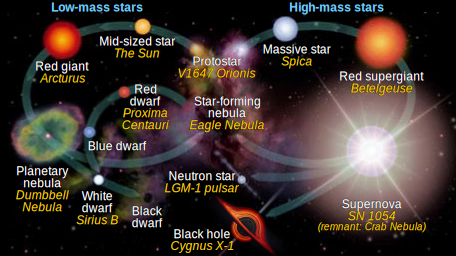
\includegraphics[width=1.0\textwidth]{Star_life_cycles.jpg}
    \caption{Lebenszyklus von leichten Sternen (links) und schweren (rechts).}
    \label{fig:Star_life_cycles}
\end{figure}

\section{Das Standardmodell der Kosmologie}
\subsection{Hubbles Gesetz}
Edwin Hubble beobachtete, dass das Spektrum aus weit entfernten Galaxien rotverschoben ist. Mit der Relativitäts-Theorie lässt sich dieser Effekt auf eine Kombination von Zeitdilatation und Längenkontraktion zurückführen. Man findet:
\begin{align*}
    \Aboxed{\te{\bf Rotverschiebung:}\quad \lambda' = \lambda\sqrt{\frac{1+\beta}{1-\beta}} \overset{\beta\ll 1}{\approx } \lambda (1+\beta)}
\end{align*}

Weiter fand Hubble einen linearen Zusammenhang zwischen Fluchgeschwindigkeit und Entfernung von Galaxien:
\begin{align*}
    \Aboxed{\te{\bf Hubble Gesetz:} \quad v = H_0 r}
\end{align*}
Wobei $H$ die \emph{Hubblekonstante} ist, welche im allgemeinen von der Zeit abhängt. Man bezeichnet die heutige Hubblekonstante mit $H_0 \approx 70 \ufrac{km/s}{Mpc}$. Das Hubblegesetz beschreibt eine überall gleich stattfindene Ausdehnung des Raumes.

\subsection{Das kosmologische Prinzip}
Das kosmologische Prinzip besagt, dass das Universum auf großen Skalen
\begin{enumerate}
    \item {\bf homogen} (gleiche Eigenschaften in jedem Punkt) ist und
    \item {\bf isotrop} (gleiche Eigenschaften in jede Richtung).
\end{enumerate}

\subsection{Friedmann-Lemaitre Gleichung}
Die Friedmann-Lemaitre Gleichung beschreibt die zeitliche Ausdehung eines homogenen isotropen Raumes mit konstanter Krümmung.
\begin{align*}
    \Aboxed{\dot R ^2 &= \frac{8\pi G}{3} \rho\sub{tot} R^2  - kc^2}
\end{align*}
Dabei beschreibt $\rho\sub{tot}=\rho\sub{Materie}+\rho\sub{Strahlung}+\rho\sub{Vakuum}$ die totale Energiedichte und $k$ die Raumkrümmung. Abhängig von $k$ gibt es drei mögliche Entwicklungen des Universums:
\begin{enumerate}
    \item $k<0\implies 0>E\sub{tot}$: Die Krümmung ist positiv wie auf einer Kugel, d.h. der Raum ist geschlossen, und das Universum wird wieder kollabieren.
    \item $k=0\implies 0=E\sub{tot}$: Das Universum ist flach, die Geometrie euklidisch und die Expansion geht asymptotisch gegen null. Nach der FL-Gleichung erfordert dies eine kritische Dichte:
    \begin{align*}
        \rho\sub{crit.} &= \frac{3H_0^2}{8\pi G} = 5.5 \ufrac{GeV}{m^3} \sim 6\ufrac{Protonen}{m^3}
    \end{align*}
    \item $k>0\implies 0<E\sub{tot}$
\end{enumerate}
Die aktuellsten Messungen von $\rho$ sind mit $\rho\sub{crit.}$ kompatibel, das Universum scheint also flach zu sein. 

\subsection{Kosmische Hintergrundstrahlung}
Die kosmologische Hintergrundstrahlung durchsetzt das gesamte Universum und folgt perfekt dem Schwarzkörperspektrum mit einer Temperatur von $(2.725\pm0.001)\u K$.
Sie entstand etwa $370,000\u a$ nach dem Urknall, als die Photonen von der Materie, mit der sie bei $\sim3000\u K$ im thermischen Gleichgewicht stand, entkoppelten.  
Da das Universum deutlich kleiner war als heute war es global im thermischen Gleichgewicht, heute misst man in der extre isotropen Strahung Fluktuationen von  von $\sim 10^{-5}$.

\section{Lerntabelle}

\begin{table}[H]
\centering
\begin{tabular}{|p{7cm}|p{7cm}|}
    \multicolumn{2}{c}{\large \bf Energieverluste}\\
    \hline
    \textbf{Frage} & \textbf{Antwort}\\\hline
    Elektronen WW nach Energie & Ionisierung dann Bremsstrahlung $E_c = \frac{560\u{MeV}}{Z}$, $\dd Ex\sub{Brems}\sim Z^2 z^2 \frac{E}{m^2}$\\\hline
    Photonen WW nach Energie& Photoeffekt $E<1\u{MeV}$, Comptoneffekt $E\sim 1\u{MeV}$, Paarbildung $E>1\u{MeV}$\\\hline 
    Hadronen WW & Starke WW\\ \hline
    Bethebloch (Anwendungsbereich, Art des Energieverlust, Proportionalität, MIP)& $\beta\gamma\in[0.1,1000]$, Anregung und Ionisation, $\frac{1}{\rho}\dd Ex\sim z^2$, $\min \frac{1}{\rho}\dd Ex = \frac{1}{\rho}\dd Ex(\beta\gamma \sim 3.5) =2\ufrac{MeV}{g/cm^2}$\\\hline
\end{tabular}
\end{table}


\begin{table}[H]
    \centering
    \begin{tabular}{|p{7cm}|p{7cm}|}
        \multicolumn{2}{c}{\large \bf Detektoren}\\
        \hline
        {\bf Frage} & {\bf Antwort}\\\hline
        Vielfachstreuung Fehler & $\sigma_\theta \sim z \sqrt x$, für kleine Winkel Gaußisch, die Ausläufer aber nicht\\\hline
        Cherenkov-Öffnungswinkel& $\cos\theta_C = \frac
        {1}{n\beta}$\\\hline
        Synchrotronstrahlung& $\Delta E\sim \frac{\gamma^4}{r}$\\\hline
        Übergangsstrahlung& $I \sim \gamma,\ \  \theta \sim \frac1 \gamma $\\\hline
        Sagitta-Messung & $\frac{\sigma_p}{p} \sim \frac{p}{B L^2}\frac{\sigma_x} {\sqrt N}$\\\hline
        ECAL & $\frac{\sigma_E}{E} \sim  \frac{1}{\sqrt{E}}$ (da $\sim \frac{\sigma_N}{N}\sim \frac{1}{\sqrt N}$)\\\hline
\end{tabular}
\end{table}

\begin{table}[H]
    \centering
    \begin{tabular}{|p{7cm}|p{7cm}|}
        \multicolumn{2}{c}{\large \bf Teilchenphysik}\\
        \hline
        {\bf Frage} & {\bf Antwort}\\\hline 
        $\hbar c$& $197\u{MeV\, fm}$\\\hline
        Spin Leptonen & $\sfrac12$\\\hline
        Spin Mesonen &\\\hline
        Spin Quark, Meson, Baryon& $\half,$ ganzzahlig, halbzahlig\\\hline
        Spin, Ladung, Masse Gluon& $\half, 0,0$\\\hline
        Spin W/Z-Boson& 0 \\\\hline
\end{tabular}
\end{table}

\begin{table}[H]
    \centering
    \begin{tabular}{|p{7cm}|p{7cm}|}
        \multicolumn{2}{c}{\large \bf Astrophysik}\\
        \hline
        {\bf Frage} & {\bf Antwort}\\\hline 
        Distanzmessungen & 1. Radar, 2. Parallaxe, 3. Standardkerzen (Cepheiden, Supernovoe vom Typ 1a, Tully-Fisher-Relation), 4. Rotverschiebung/Hubblegesetz \\\hline
        Hertzsprung-Russel-Diagram & $x:1/T$, $y:L$\\\hline
        Stern Lebenszyklen& siehe Grafik \ref{fig:Star_life_cycles} \\\hline
        Friedmann-Lemaitre& $\dot R ^2 = \frac{8\pi G}{3} \rho\sub{tot} R^2  - kc^2$, $R\hat = $Radius Universum, $k\hat =$Krümmung (positiv$\leftrightarrow$Erde)\\\hline
        Hubble Parameter & $H=\dot R/R$\\\hline
        &\\\hline
\end{tabular}
\end{table}


\end{document}